\section{A Budget--Stakes Law: What a Sublinear Test Can and Cannot
Buy}

Every experiment above met the same wall: on average-case matching the
advice-free baseline is near-optimal, so predictions buy robustness
insurance rather than performance, and --- for the test-and-fallback
algorithms --- no acceptance threshold both captures the (tiny) upside
and stays safe (§5.3). This section quantifies the wall. The result is a
two-sided \textbf{budget--stakes law}: on a natural instance family,
deciding whether to follow the advice requires a prefix of length
\(k^* = \tilde\Theta(\theta/\delta^2)\) --- the inverse square of the
stakes \(\delta\), scaled by the contention \(\theta\) --- and this is
\emph{sharp}: below \(k^*\) \textbf{no} decision rule whatsoever can be
simultaneously consistent and robust (Theorem 1(i)), while at \(k^*\) an
explicit, embarrassingly simple rule succeeds (Theorem 1(ii)). The
corollary is the wall: stakes are capped by the baseline slack, so on
strong-baseline instances the required prefix exceeds the entire horizon
--- any upside smaller than
\(\approx 2\sqrt{(1-\rho_{\mathrm{base}})/n}\) is uncapturable at
\emph{every} \(k\le n\), and the upsides we measured in §3--§5 sit in
exactly that range.

En route we record an honest negative of independent interest (§7.7):
the natural conjecture --- that the \(\tilde\Theta(r/\log r)\) hardness
of \emph{tolerant distribution testing}
\cite{canonne2022tolerance,valiant2011unseen,jiao2018l1} makes the
follow/fallback decision itself hard for any rule at sublinear \(k\) ---
is \textbf{false}. The advice's \emph{distance} \(\ell_1(p,q)\) is
indeed hard to test, and the empirical-\(\ell_1\) rules the field
actually uses \cite{choo2024imperfect,bem2026testmatch} are provably
blind at \(k \ll r\); but the decision-relevant functional is the
\emph{payoff} of following, which on decomposable instances collapses to
a per-sample observable. Testing the payoff is exponentially cheaper
than testing the prediction.

\textbf{Relation to prior work.} Choo et al.~\cite{choo2024imperfect}
and Burathep--Erlebach--Moses \cite{bem2026testmatch} give \emph{upper}
bounds (algorithms) in this model and no statistical lower bound; Choo
et al.'s Thm 3.1 is the generic adversarial trade-off (no algorithm is
\(1\)-consistent and \(>\tfrac12\)-robust), driven by adversarial
instances, not by the resolution of a sublinear test. Their acceptance
threshold \(\tau = 2(\hat n/n-\beta)-\varepsilon\) couples to the
baseline \(\beta\) \emph{constructively}; Theorem 1(i) is the
information-theoretic counterpart --- it binds \emph{every} measurable
rule on the prefix. The consistency/robustness lower bounds elsewhere in
the with-predictions literature \cite{weizhang2020tradeoffs} are
problem-intrinsic Pareto frontiers, not gated by a test.
Tolerant-testing sample complexity \cite{canonne2022tolerance} enters
our story twice, both times off the critical path: it explains
\emph{why} the field's \(\ell_1\)-threshold rules are blind (§7.7), and
its hard instances are exactly what our payoff identity (Lemma 2)
sidesteps. To our knowledge, both the budget--stakes law and the
observation that payoff-testing strictly separates from distance-testing
in an online algorithm are new; a dedicated literature pass on
payoff-estimating acceptance rules is in progress.

\subsection{The test-and-fallback
class}

Fix an instance family and a budget \(k=o(n)\). A
\textbf{test-and-fallback} algorithm \(A_k\) observes the first \(k\)
arrivals \(X_{1:k}\) and the advice \(\sigma\), outputs a (possibly
randomized) decision \(D\in\{\mathsf{Follow},\mathsf{Fallback}\}\) as a
function of \((X_{1:k},\sigma)\), and thereafter Mimics \(\sigma\) if
\(D=\mathsf{Follow}\) and runs the advice-free baseline \(B\) (Ranking)
otherwise. Because \(k=o(n)\), the prefix's own contribution to the
ratio is \(O(k/n)=o(1)\), absorbed below. Write \(\rho_{\mathrm{base}} =
\mathbb E[B]/\mathrm{OPT}\) for the baseline strength,
\textbf{consistency} for the ratio under good advice, and
\textbf{robustness} for the ratio under adversarial advice.

\subsection{The master trade-off
(rigorous)}

\begin{quote}
\textbf{Lemma 1.} Let \(G,\mathrm{Bd}\) be two instance distributions
sharing the \emph{same} advice \(\sigma\), with prefix laws
\(\mathcal L_G,\mathcal L_{\mathrm{Bd}}\) and
\(\gamma_k:=\mathrm{TV}(\mathcal L_G,\mathcal L_{\mathrm{Bd}})\).
Suppose following \(\sigma\) gains \(\delta\) under \(G\) and loses
\(\Delta\) under \(\mathrm{Bd}\) relative to \(B\). Parameterize \(A_k\)
by the fraction \(\eta_c\) of the upside it forgoes under \(G\) and its
robustness loss \(\eta_r\Delta\) under \(\mathrm{Bd}\). Then
\[(1-\eta_c)\;\le\;\eta_r+\gamma_k+o(1).\]
\end{quote}

\emph{Proof.} Conditioning on \(D\) under \(G\),
\(\mathbb E_G[A_k]/\mathrm{OPT} = P_G(\mathsf F)\,
\mathbb E_G[\mathrm{Mimic}]/\mathrm{OPT} + P_G(\mathsf R)\rho_{\mathrm{base}} \pm o(1) \ge
\rho_{\mathrm{base}} + \delta\,P_G(\mathsf F)-o(1)\), so the captured
upside \((1-\eta_c)\delta\) forces \(P_G(\mathsf F)\ge 1-\eta_c-o(1)\).
Symmetrically \(P_{\mathrm{Bd}}(\mathsf F)=\eta_r
+o(1)\). Since \(D\) is a function of \((X_{1:k},\sigma)\) and
\(\sigma\) is identical,
\(|P_G(\mathsf F)-P_{\mathrm{Bd}}(\mathsf F)|\le\gamma_k\); chaining
gives the claim. \(\qed\)

With an \emph{uninformative} prefix (\(\gamma_k=o(1)\)) one cannot be
both near-fully-consistent (\(\eta_c\to0\)) and robust (\(\eta_r\to0\)).
Everything below is a computation of how large \(k\) must be before the
prefix becomes informative --- and (the half the earlier draft missed)
of how \emph{small} a \(k\) already suffices.

\subsection{The construction and the affine
law}

The family is a disjoint union of \(m\) independent
\textbf{rare-resource cells}, each over a distinct type-pair, so the
support is \(r=\Theta(m)\) and (at \(m = \Theta(n)\)) each type is seen
\(O(1)\) times. A cell has resources \(\{a_i,b_i\}\), a flexible request
(neighborhood \(\{a_i,b_i\}\)) that must be routed before a specialist
(\(\{a_i\}\) or \(\{b_i\}\), present with probability \(\theta\)) is
seen; the right route depends on the future specialist. In closed form
(verified numerically), per cell \(\mathrm{OPT}=1+\theta\), baseline
\(=1+\theta/2\), and following the advice gains or loses exactly
\(\theta\lvert s-\tfrac12\rvert\) over the baseline according to whether
the advice's \emph{direction} is right, where
\(s = \tfrac12 \pm \varepsilon\) is the specialist bias and
\(\varepsilon\) the signal; the advice-to-truth distance is
\(\ell_1=2\theta\lvert s-\hat s\rvert\) per cell.

These aggregate cleanly. Summing over cells yields an \textbf{exact
affine law} (proven; verified to three decimals):
\[\mathbb E[\text{follow-ratio}] \;=\; \rho_{\mathrm{perfect}} - \tfrac12\,\ell_1(p,q),
\qquad \ell_1^\star \;=\; 2\big(\rho_{\mathrm{perfect}}-\rho_{\mathrm{base}}\big),\]
where \(\rho_{\mathrm{perfect}}\) is the all-correct-direction ratio and
\(\ell_1^\star\) the break-even. Two identities anchor what follows: the
baseline slack is
\(1-\rho_{\mathrm{base}} = \tfrac{\theta}{2(1+\theta)}\), and the
maximum stakes (the full upside) are
\[\rho_{\mathrm{perfect}}-\rho_{\mathrm{base}} \;=\; \frac{\theta\varepsilon}{1+\theta}
\;=\; 2\varepsilon\,(1-\rho_{\mathrm{base}}):\] \emph{the upside is an
\(\varepsilon\)-fraction of the baseline slack.} The canonical scenario
pair takes a wrong-direction fraction \(\varphi=\tfrac14\) (good:
\(\ell_1 = a\), gain \(\delta\)) versus \(\varphi=\tfrac34\) (bad:
\(\ell_1 = b\), loss \(\Delta\)), with \(\delta=\Delta=\ell_1^\star/4\).

\subsection{The payoff identity: the stakes are a per-sample
observable}

The earlier route tried to make the follow/fallback decision \emph{hard}
by making \(\ell_1(p,q)\) hard to test. On this family that cannot work,
for a reason worth a lemma. Classify each arrival by its role in its own
cell, relative to the advice's predicted direction:
\[c(X) \;=\; \begin{cases} +1 & X \text{ is the advice-favored specialist of its cell,} \\
-1 & X \text{ is the disfavored specialist,} \\ 0 & X \text{ is flexible.}\end{cases}\]

\begin{quote}
\textbf{Lemma 2 (payoff identity).} For every type distribution \(p\) in
the family,
\[\mathbb E_p[c] \;=\; 2\cdot\frac{\mathbb E_p[\mathrm{Mimic}]-\mathbb E_p[B]}{\mathrm{OPT}}.\]
\emph{The expected advantage of following the advice is half the mean of
a bounded, per-sample observable.} (Verified to three decimals across
all wrong-fractions; \texttt{scripts/verify\_witness\_gap.py}.)
\end{quote}

\emph{Proof.} The favored and disfavored specialists of cell \(i\) have
masses \(\theta(\tfrac12\pm\varepsilon d_i\hat d_i)/N\), where
\(d_i,\hat d_i\) are the truth and advice directions and
\(N=m(1+\theta)=\mathrm{OPT}\); so cell \(i\) contributes
\(2\theta\varepsilon d_i\hat d_i/N\) to \(\mathbb E[c]\), while by the
cell constants its follow-advantage is
\(\theta\varepsilon d_i\hat d_i\). Sum over cells. \(\qed\)

\subsection{The budget--stakes law}

\begin{quote}
\textbf{Theorem 1 (budget--stakes law).} On the cell family with
contention \(\theta\), signal \(\varepsilon\), and the canonical
scenario pair with stakes \(\delta=\Delta\):

\textbf{(i) (Impossibility below the budget --- any rule.)} If
\(k \,=\, o\!\big(\theta/\delta^2\big)\) \emph{(equivalently
\(o\big((1{+}\theta)/(\theta\varepsilon^2)\big)\))}, then every
test-and-fallback algorithm \(A_k\), deciding by \emph{any} measurable
rule on the prefix, has \(\eta_c+\eta_r \ge 1-o(1)\): it forgoes the
upside or eats the loss.

\textbf{(ii) (The budget suffices --- an explicit rule.)} The
\textbf{directional test} --- follow iff \(\sum_{j\le k} c(X_j) > 0\)
--- achieves \(\eta_c+\eta_r \le \epsilon_0\) once
\(k \ge C\,(\theta/\delta^2)\log(1/\epsilon_0)\). In particular \(k\) is
\emph{independent of \(n\)} for constant error.

Hence the critical budget is \(k^* = \tilde\Theta(\theta/\delta^2)\).
\end{quote}

\emph{Proof of (ii).} Under the good scenario \(\mathbb E[c] = 2\delta\)
(Lemma 2), under the bad \(-2\Delta\);
\(\mathrm{Var}(c) \le \mathbb P(\text{specialist}) = \theta/(1+\theta)\);
Bernstein's inequality gives error \(\exp(-\Omega(k\delta^2/\theta))\)
on both sides. \(\qed\)

\emph{Proof sketch of (i).} Couple the two scenarios so their direction
vectors differ on a \(\tfrac12\)-fraction of cells. For a coupled pair
of fixed direction vectors, the per-sample laws differ only on the
specialists of differing cells, giving squared Hellinger distance
\(H^2_{\mathrm{per}} = \Theta(\theta\varepsilon^2)\); by tensorization
and joint convexity,
\(\gamma_k \le \sqrt{2k\,H^2_{\mathrm{per}}} = o(1)\) whenever
\(k = o(1/(\theta\varepsilon^2))\). Lemma 1 then forces
\(\eta_c+\eta_r\ge 1-o(1)\). Since
\(\delta = \Theta(\theta\varepsilon)\), the two thresholds match up to
the stated factors. \(\qed\)

Numerically (§\texttt{verify\_witness\_gap.py}, \(\theta=0.6\),
\(\varepsilon=0.3\), \(\delta=0.056\)): the directional test reaches
\(\eta_c+\eta_r \approx 0.06\) at \(k=100\) and \(0.007\) at \(k=200\),
and stays flat as \(n\) grows from \(3{,}200\) to \(320{,}000\) at fixed
\(k=200\) --- the budget really is \(n\)-free once the stakes are
constant.

\subsection{The wall, quantified: strong baselines price the test out of
the
horizon}

Stakes are capped by the slack:
\(\delta \le \rho_{\mathrm{perfect}}-\rho_{\mathrm{base}} =
2\varepsilon(1-\rho_{\mathrm{base}})\). Substituting into Theorem 1(i),
capturing \emph{any} constant fraction of the maximum upside requires
\[k \;\ge\; \tilde\Omega\!\Big(\frac{\theta}{\varepsilon^2(1-\rho_{\mathrm{base}})^2}\Big)
\;=\; \tilde\Omega\!\Big(\frac1{\varepsilon^2\,(1-\rho_{\mathrm{base}})}\Big),\]
using \(\theta = \Theta(1-\rho_{\mathrm{base}})\). The wall appears when
this exceeds the horizon itself: \(k^* \ge n\) exactly when the upside
\(2\varepsilon(1-\rho_{\mathrm{base}})\) falls below
\(\approx 2\sqrt{(1-\rho_{\mathrm{base}})/n}\). In words:

\begin{quote}
\textbf{Corollary (uncapturable upsides).} On strong-baseline families,
every advice upside smaller than
\(\Theta\big(\sqrt{(1-\rho_{\mathrm{base}})/n}\,\big)\) is uncapturable
by any test-and-fallback rule at any prefix length \(k \le n\) --- the
information needed to decide does not exist inside the instance.
\end{quote}

At the parameters of our benchmark (§3:
\(\rho_{\mathrm{base}}\approx0.99\), \(n=2000\)) the threshold is
\(\approx 0.004\), and the measured upsides are \(<0.01\) (F3) --- the
empirical wall sits in the regime the corollary governs. This is the
\textbf{scissors} of \textbf{Figure 7}
(\texttt{results/impossibility\_frontier.png}), now with the correct
mechanism: the \emph{potential} upside (perfect advice minus baseline)
grows as the baseline weakens, while the upside a feasible test can
safely capture is pinned by the \(\sqrt{(1-\rho_{\mathrm{base}})/n}\)
resolution --- \textbf{the structure that makes the baseline strong is
the structure that starves the test of signal.}

\begin{figure}
\centering
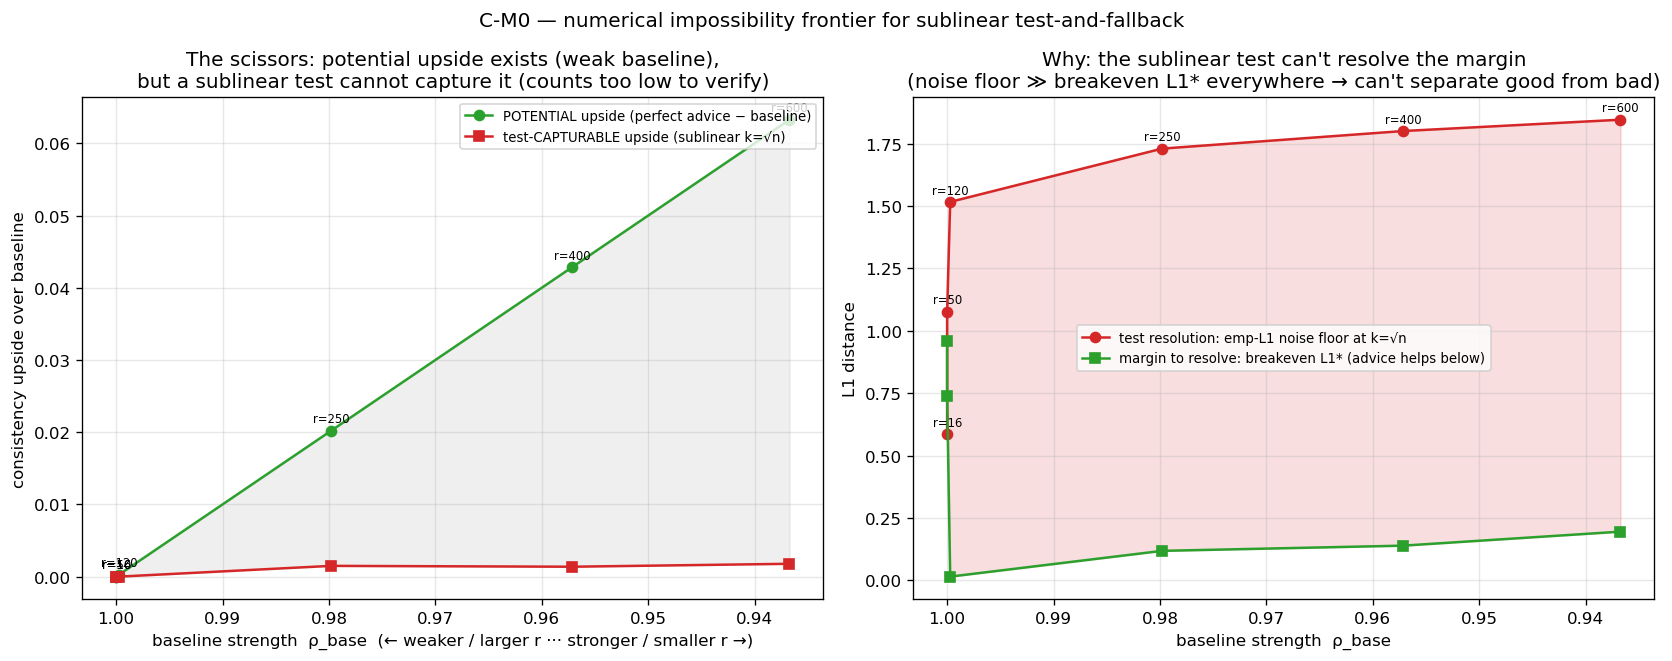
\includegraphics[width=1\linewidth,height=\textheight,keepaspectratio,alt={The budget--stakes scissors: as the baseline weakens (left), the potential upside of perfect advice grows, while the upside a feasible test can safely capture stays pinned near zero --- the empirical test's resolution sits far above the break-even margin wherever the upside exists.}]{../../../results/impossibility_frontier.png}
\caption{The budget--stakes scissors: as the baseline weakens (left),
the potential upside of perfect advice grows, while the upside a
feasible test can safely capture stays pinned near zero --- the
empirical test's resolution sits far above the break-even margin
wherever the upside exists.}
\end{figure}

\subsection{Why the field's rules hit the wall earlier: distance-testing
is the wrong
statistic}

The algorithms of \cite{choo2024imperfect,bem2026testmatch} do not run
the directional test; they threshold the plug-in distance
\(\hat\ell_1(\hat p_k, q)\). That class is blind far before Theorem 1(i)
bites: at \(k \ll r\) the empirical \(\hat p_k\) is \(k\) atoms of mass
\(1/k\), so \(\hat\ell_1 \approx 2\) \emph{regardless of the advice's
quality} (numerically: \(1.908\) vs \(1.913\) on the two canonical
scenarios whose true \(\ell_1\) differ by \(0.225\)). Any threshold
therefore either always accepts or always rejects --- the §5.3
pathology, now explained. The deeper reason is the tolerant-testing
barrier: estimating \(\ell_1(p,q)\) to constant accuracy at
\(r=\Theta(n)\) genuinely requires \(\tilde\Theta(n/\log n)\) samples
\cite{canonne2022tolerance}. The resolution of the apparent paradox ---
the \emph{decision} is easy (Theorem 1(ii)) while the \emph{distance} is
hard --- is Lemma 2: the payoff is a linear, per-sample functional, and
\(\ell_1\) is not. The practical moral for algorithm designers is one
sentence: \textbf{test the payoff, not the prediction.}

We record the flip side honestly. The natural conjecture behind an
earlier version of this section --- that tolerant-testing hardness makes
the follow/fallback decision itself impossible for \emph{any} rule at
\(k = o(n/\log n)\) with \(\Theta(1)\) stakes --- is \textbf{refuted} by
Theorem 1(ii): no witness pair with \(\gamma_k = o(1)\) and
\(\Theta(1)\) stakes exists on this family, because by Lemma 2 a
\(\Theta(1)\) stake gap forces \(\gamma_k \to 1\) at any
\(k=\omega(1)\). The tolerant-testing hard instances evade Lemma 2 only
by mismatching the advice's per-cell magnitudes --- precisely the regime
in which distance and payoff decouple and \(\ell_1\) stops being the
decision-relevant quantity.

\subsection{Scope and honesty}

Both halves of Theorem 1 use only elementary tools (Bernstein; Hellinger
tensorization plus Lemma 1) --- deliberately: the earlier,
stronger-sounding route through tolerant-testing lower bounds is closed
by §7.7, and we consider the refutation itself part of the contribution.
The law is stated for decomposable (disjoint-cell) families; by Lemma 2
the payoff is per-sample observable on \emph{every} such family, so no
decomposable construction can restore a super-\(1/\delta^2\) barrier.
Whether a \emph{non-decomposable} family --- long-range dependence
making the payoff a genuinely hard functional --- can separate the
budget from \(1/\delta^2\) is open. The directional test is analyzed
here only on the cell family; its novelty relative to payoff-estimating
switching rules elsewhere in the learning-augmented literature is under
a dedicated literature pass. We credit Choo et al.~for the constructive
baseline-coupling their threshold already exhibits; our contribution is
the two-sided, rule-independent budget law, the payoff/distance
separation, and the quantified wall.
